\section{Test Results}
In this section, we test the proposed techinque on the use case explained in the previouse section.

\subsection{Verification of Results}
It is imporant to verify that the results obtained from the simulator actually matches real-world observations.
Figure~\ref{} and~\ref{} show data from ???.

From Figure~\ref{fig:TestResults:distance0} we see that the simulation compared to the real-world results from Figure \ref{} is a close match. 
We see the same stop and go behavior as a results from traffic lights, and the arrival times are also a close match. 
If we compare the driving speed of the simulation show in Figure \ref{fig:TestResults:speed0} with the real-world data from Figure \ref{} we see that in most cases the vehicles are either driving at the maximum speed, or they are at a full stop. 
This behavior on the two graphs are almost identical and consistent with the stop and go behavior caused by traffic lights. 
Figure \ref{} shows the distance to a traffic light where each vehicles makes a stop. 
All the blue dots are vehicles that only have a single stop, red squares have two stops and yellow triangles have 3 stops.
The traffic light for this figure is the first junctions driving from Vesterbro. See Figure \ref{fig:Introduction:hobro}. The Figure \ref{} show the real-world data from the same traffic light. 
%TODO: when we have something to compare with

\begin{figure}[htb]
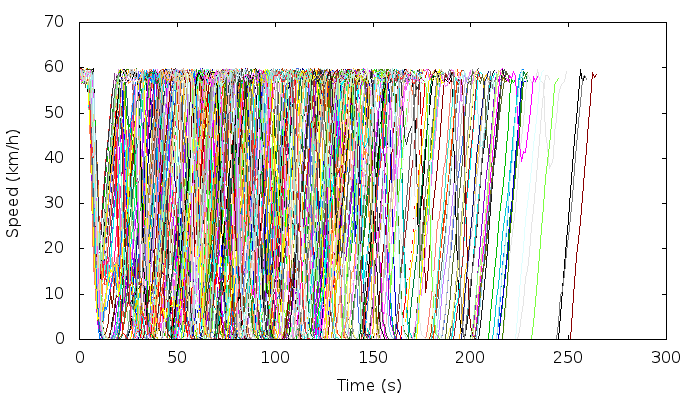
\includegraphics[width=0.5\textwidth]{images/tp0/speedUncontrolled0.png}
\caption{Speed graph}
\label{fig:TestResults:speed0}
\end{figure}

\begin{figure}[htb]
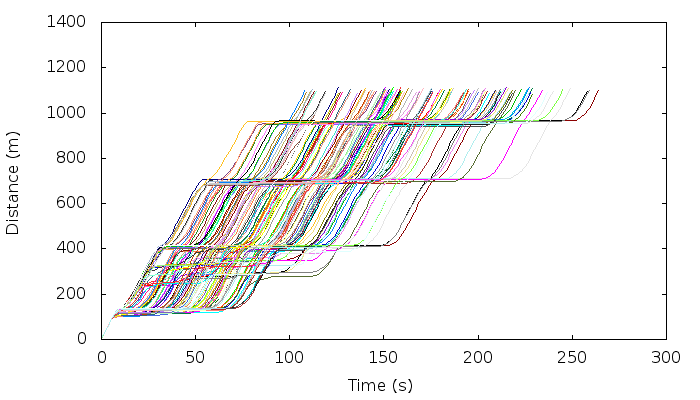
\includegraphics[width=0.5\textwidth]{images/tp0/distanceUncontrolled0.png}
\caption{Distance graph}
\label{fig:TestResults:distance0}
\end{figure}

%
\begin{figure}
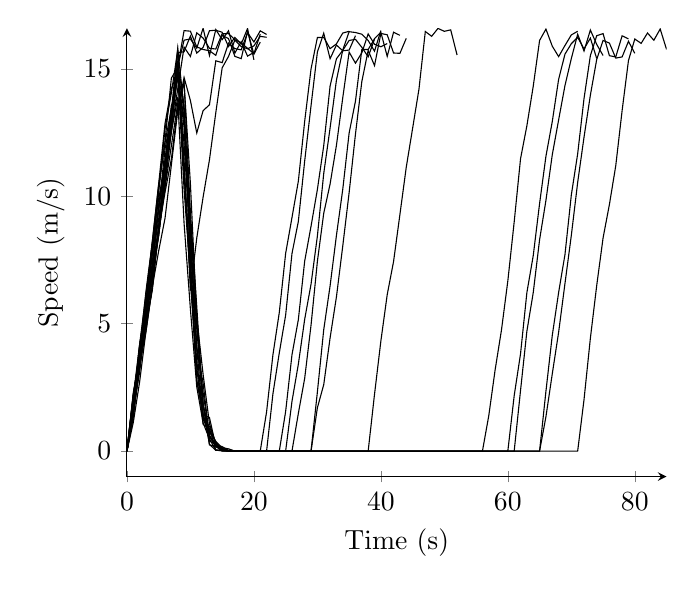
\begin{tikzpicture}
\begin{axis}[
legend style={anchor=west},
axis x line=bottom,
axis y line=left,
ymin=-1,
xlabel=Time (s),
ylabel=Speed (m/s),
]
\addplot[] coordinates {
(0, 0.0)
(1, 1.69655878999)
(2, 3.67956839706)
(3, 5.19272490987)
(4, 7.20356419508)
(5, 8.5737242637)
(6, 10.7899166882)
(7, 12.5081667572)
(8, 14.2099448128)
(9, 15.8518676442)
(10, 15.4860138311)
(11, 16.4121611704)
(12, 16.2075640619)
(13, 15.805771308)
(14, 15.7770029409)
(15, 16.376577111)
(16, 16.379913727)
(17, 16.1471423445)
(18, 16.0138479285)
(19, 15.8056926081)
(20, 15.5941200483)
(21, 16.3613227376)
};
\addplot[] coordinates {
(0, 0.0)
(1, 2.21121398936)
(2, 3.59285451821)
(3, 5.45790431643)
(4, 7.08020272548)
(5, 9.53823663498)
(6, 11.4596679897)
(7, 13.3623035229)
(8, 14.8760363605)
(9, 12.0485909913)
(10, 8.1243544415)
(11, 4.04465906846)
(12, 1.29806627542)
(13, 0.965862562495)
(14, 0.318337276114)
(15, 0.0815088310026)
(16, 0.0203345879742)
(17, 0.0)
(18, 0.0)
(19, 0.0)
(20, 0.0)
(21, 0.0)
(22, 0.0)
(23, 0.0)
(24, 0.0)
(25, 1.55413603643)
(26, 3.77907186659)
(27, 5.15578950755)
(28, 7.45418968872)
(29, 8.82250386494)
(30, 10.2651877131)
(31, 11.9845689784)
(32, 14.3253558327)
(33, 15.3939306363)
(34, 15.7255389416)
(35, 16.1136710649)
(36, 16.1571932173)
(37, 15.8447128613)
(38, 15.4723728657)
(39, 16.1609261253)
};
\addplot[] coordinates {
(0, 0.0)
(1, 1.57429128769)
(2, 3.53650107689)
(3, 4.99217562319)
(4, 6.44208426325)
(5, 7.85435972153)
(6, 9.13540175854)
(7, 11.2277544598)
(8, 13.3369616038)
(9, 14.6629914441)
(10, 13.7562936201)
(11, 12.4838164913)
(12, 13.3583665095)
(13, 13.5890204041)
(14, 15.3150675343)
(15, 15.2439689759)
(16, 16.0071006542)
(17, 15.793851726)
(18, 15.7440448308)
(19, 16.4194145001)
(20, 16.0551274081)
(21, 16.4913308166)
(22, 16.3489043325)
};
\addplot[] coordinates {
(0, 0.0)
(1, 1.59891751121)
(2, 3.98457542112)
(3, 6.27387736363)
(4, 8.19742514482)
(5, 10.4383861724)
(6, 12.0936067899)
(7, 13.4403211308)
(8, 14.8479898922)
(9, 10.9908702879)
(10, 7.30053526354)
(11, 3.29626058053)
(12, 1.04572542945)
(13, 0.883870550075)
(14, 0.0496195717564)
(15, 0.0259550926758)
(16, 0.0161643831833)
(17, 0.0)
(18, 0.0)
(19, 0.0)
(20, 0.0)
(21, 0.0)
(22, 0.0)
(23, 0.0)
(24, 0.0)
(25, 0.0)
(26, 0.0)
(27, 0.0)
(28, 0.0)
(29, 0.0)
(30, 0.0)
(31, 0.0)
(32, 0.0)
(33, 0.0)
(34, 0.0)
(35, 0.0)
(36, 0.0)
(37, 0.0)
(38, 0.0)
(39, 2.22701815801)
(40, 4.31829619425)
(41, 6.13777380728)
(42, 7.43947288312)
(43, 9.28266234085)
(44, 11.1397831561)
(45, 12.6635801216)
(46, 14.2016706953)
(47, 16.4656396166)
(48, 16.2764431518)
(49, 16.5862954565)
(50, 16.4718890772)
(51, 16.5296137568)
(52, 15.5456225908)
};
\addplot[] coordinates {
(0, 0.0)
(1, 1.44117465738)
(2, 3.44338031864)
(3, 5.28968274622)
(4, 7.29384729726)
(5, 9.67850462795)
(6, 11.1405541011)
(7, 12.6398144106)
(8, 14.9880648046)
(9, 13.3379256958)
(10, 7.78188122213)
(11, 5.1435470078)
(12, 1.86518108958)
(13, 0.242447056624)
(14, 0.187500411133)
(15, 0.0139345132501)
(16, 0.0)
(17, 0.0)
(18, 0.0)
(19, 0.0)
(20, 0.0)
(21, 0.0)
(22, 1.5402096021)
(23, 3.78246421518)
(24, 5.43688386446)
(25, 7.7562591451)
(26, 9.16652720276)
(27, 10.5898654248)
(28, 12.9424510061)
(29, 14.9969998465)
(30, 16.2278432352)
(31, 16.2351880036)
(32, 15.7912144583)
(33, 15.9791797187)
(34, 16.4046871013)
(35, 16.4727939988)
};
\addplot[] coordinates {
(0, 0.0)
(1, 2.12616742007)
(2, 4.19329186872)
(3, 5.6919135229)
(4, 7.89838829078)
(5, 10.2796010577)
(6, 12.1599819956)
(7, 14.6357143813)
(8, 15.0528237228)
(9, 11.4158128506)
(10, 6.297614139)
(11, 8.35899559487)
(12, 9.96607545993)
(13, 11.432352401)
(14, 13.2800165118)
(15, 15.0379895419)
(16, 15.4857963213)
(17, 16.1255716614)
(18, 15.8771209058)
(19, 15.7861428542)
(20, 15.9017509198)
(21, 16.2739378924)
(22, 16.2391567355)
};
\addplot[] coordinates {
(0, 0.0)
(1, 1.93305703113)
(2, 4.13554966013)
(3, 5.72500893526)
(4, 8.0593960773)
(5, 9.46967692056)
(6, 11.854418639)
(7, 13.1735351184)
(8, 15.6387967503)
(9, 15.669845863)
(10, 16.2888681309)
(11, 15.6172210126)
(12, 15.842290706)
(13, 16.4945108891)
(14, 16.5160755018)
(15, 16.4343506109)
(16, 15.8733656333)
(17, 16.2335178043)
(18, 15.9711069616)
(19, 16.5846852335)
(20, 15.3518956352)
};
\addplot[] coordinates {
(0, 0.0)
(1, 1.72800719243)
(2, 3.55822897458)
(3, 5.55445920385)
(4, 7.80072680674)
(5, 10.1552350406)
(6, 12.6490986621)
(7, 14.0492980054)
(8, 15.7339862424)
(9, 11.087762116)
(10, 7.23641608203)
(11, 2.78237483288)
(12, 1.43614198184)
(13, 0.394618942235)
(14, 0.265801609592)
(15, 0.0420118674928)
(16, 0.011768430675)
(17, 0.0)
(18, 0.0)
(19, 0.0)
(20, 0.0)
(21, 0.0)
(22, 0.0)
(23, 0.0)
(24, 0.0)
(25, 0.0)
(26, 0.0)
(27, 0.0)
(28, 0.0)
(29, 0.0)
(30, 0.0)
(31, 0.0)
(32, 0.0)
(33, 0.0)
(34, 0.0)
(35, 0.0)
(36, 0.0)
(37, 0.0)
(38, 0.0)
(39, 0.0)
(40, 0.0)
(41, 0.0)
(42, 0.0)
(43, 0.0)
(44, 0.0)
(45, 0.0)
(46, 0.0)
(47, 0.0)
(48, 0.0)
(49, 0.0)
(50, 0.0)
(51, 0.0)
(52, 0.0)
(53, 0.0)
(54, 0.0)
(55, 0.0)
(56, 0.0)
(57, 1.3926015349)
(58, 3.18965922255)
(59, 4.7542434599)
(60, 6.68003495724)
(61, 8.99055800546)
(62, 11.4714384041)
(63, 12.7666285957)
(64, 14.3153023391)
(65, 16.1122029411)
(66, 16.559530771)
(67, 15.8895344371)
(68, 15.4795046508)
(69, 15.9167218118)
(70, 16.330392858)
(71, 16.4747433422)
};
\addplot[] coordinates {
(0, 0.0)
(1, 2.15391133737)
(2, 3.92069633061)
(3, 5.68047448178)
(4, 7.01535401953)
(5, 8.43687932327)
(6, 10.6935469003)
(7, 12.7973568795)
(8, 14.7339270296)
(9, 13.0211991519)
(10, 8.67103513938)
(11, 4.11339048306)
(12, 2.2963351297)
(13, 0.580072811148)
(14, 0.282998586036)
(15, 0.0863961507886)
(16, 0.0)
(17, 0.0)
(18, 0.0)
(19, 0.0)
(20, 0.0)
(21, 0.0)
(22, 0.0)
(23, 0.0)
(24, 0.0)
(25, 0.0)
(26, 0.0)
(27, 0.0)
(28, 0.0)
(29, 0.0)
(30, 0.0)
(31, 0.0)
(32, 0.0)
(33, 0.0)
(34, 0.0)
(35, 0.0)
(36, 0.0)
(37, 0.0)
(38, 0.0)
(39, 0.0)
(40, 0.0)
(41, 0.0)
(42, 0.0)
(43, 0.0)
(44, 0.0)
(45, 0.0)
(46, 0.0)
(47, 0.0)
(48, 0.0)
(49, 0.0)
(50, 0.0)
(51, 0.0)
(52, 0.0)
(53, 0.0)
(54, 0.0)
(55, 0.0)
(56, 0.0)
(57, 0.0)
(58, 0.0)
(59, 0.0)
(60, 0.0)
(61, 0.0)
(62, 0.0)
(63, 0.0)
(64, 0.0)
(65, 0.0)
(66, 0.0)
(67, 0.0)
(68, 0.0)
(69, 0.0)
(70, 0.0)
(71, 0.0)
(72, 2.01908573479)
(73, 4.42585163808)
(74, 6.49724935094)
(75, 8.36174359778)
(76, 9.67761302018)
(77, 11.1979801283)
(78, 13.3601725296)
(79, 15.3238696061)
(80, 16.1702353035)
(81, 15.9989677579)
(82, 16.4057737105)
(83, 16.1208111173)
(84, 16.5637219947)
(85, 15.7610954609)
};
\addplot[] coordinates {
(0, 0.0)
(1, 1.56946584146)
(2, 3.09415850206)
(3, 5.13459491602)
(4, 6.70768423559)
(5, 8.45885561605)
(6, 10.6505276111)
(7, 13.1024183906)
(8, 15.2725959348)
(9, 13.5691848483)
(10, 8.79965043157)
(11, 5.29816334608)
(12, 1.77933855823)
(13, 0.622337701857)
(14, 0.233352224777)
(15, 0.176862404631)
(16, 0.0194313604896)
(17, 0.0)
(18, 0.0)
(19, 0.0)
(20, 0.0)
(21, 0.0)
(22, 0.0)
(23, 0.0)
(24, 0.0)
(25, 0.0)
(26, 1.95257699525)
(27, 3.4067007812)
(28, 5.17198963236)
(29, 6.5479420044)
(30, 8.43751423468)
(31, 10.891402156)
(32, 12.6752913179)
(33, 14.5514645832)
(34, 15.7399044552)
(35, 16.4574820848)
(36, 16.4251046459)
(37, 16.3598376629)
(38, 16.1124643348)
(39, 15.6938809124)
(40, 16.5001951495)
};
\addplot[] coordinates {
(0, 0.0)
(1, 1.76217175409)
(2, 3.95900752424)
(3, 5.88440275606)
(4, 8.238239036)
(5, 10.4874022488)
(6, 12.8510501594)
(7, 14.2197145952)
(8, 14.8875235286)
(9, 10.2819409787)
(10, 6.85276609781)
(11, 2.75159340453)
(12, 1.43282266635)
(13, 0.61206581378)
(14, 0.166196718036)
(15, 0.0960943362038)
(16, 0.0)
(17, 0.0)
(18, 0.0)
(19, 0.0)
(20, 0.0)
(21, 0.0)
(22, 0.0)
(23, 0.0)
(24, 0.0)
(25, 0.0)
(26, 0.0)
(27, 0.0)
(28, 0.0)
(29, 0.0)
(30, 0.0)
(31, 0.0)
(32, 0.0)
(33, 0.0)
(34, 0.0)
(35, 0.0)
(36, 0.0)
(37, 0.0)
(38, 0.0)
(39, 0.0)
(40, 0.0)
(41, 0.0)
(42, 0.0)
(43, 0.0)
(44, 0.0)
(45, 0.0)
(46, 0.0)
(47, 0.0)
(48, 0.0)
(49, 0.0)
(50, 0.0)
(51, 0.0)
(52, 0.0)
(53, 0.0)
(54, 0.0)
(55, 0.0)
(56, 0.0)
(57, 0.0)
(58, 0.0)
(59, 0.0)
(60, 0.0)
(61, 2.17250207817)
(62, 3.81653779303)
(63, 6.22125260328)
(64, 7.66564355261)
(65, 9.71165935218)
(66, 11.5674470877)
(67, 12.9311783827)
(68, 14.5882285229)
(69, 15.5764424524)
(70, 15.9871104351)
(71, 16.2367633803)
(72, 15.7811718294)
(73, 16.2054076054)
(74, 15.4049100628)
};
\addplot[] coordinates {
(0, 0.0)
(1, 2.28535288596)
(2, 3.70210856199)
(3, 5.52483096719)
(4, 7.71647389338)
(5, 9.45676035044)
(6, 11.2365432421)
(7, 12.5545747174)
(8, 13.8425897987)
(9, 13.2098117887)
(10, 7.46539523987)
(11, 4.01294297319)
(12, 2.66552671691)
(13, 0.537530884295)
(14, 0.227326585301)
(15, 0.0376341870259)
(16, 0.0135643362328)
(17, 0.0)
(18, 0.0)
(19, 0.0)
(20, 0.0)
(21, 0.0)
(22, 0.0)
(23, 0.0)
(24, 0.0)
(25, 0.0)
(26, 0.0)
(27, 0.0)
(28, 0.0)
(29, 0.0)
(30, 0.0)
(31, 0.0)
(32, 0.0)
(33, 0.0)
(34, 0.0)
(35, 0.0)
(36, 0.0)
(37, 0.0)
(38, 0.0)
(39, 0.0)
(40, 0.0)
(41, 0.0)
(42, 0.0)
(43, 0.0)
(44, 0.0)
(45, 0.0)
(46, 0.0)
(47, 0.0)
(48, 0.0)
(49, 0.0)
(50, 0.0)
(51, 0.0)
(52, 0.0)
(53, 0.0)
(54, 0.0)
(55, 0.0)
(56, 0.0)
(57, 0.0)
(58, 0.0)
(59, 0.0)
(60, 0.0)
(61, 0.0)
(62, 2.37832577695)
(63, 4.70544832642)
(64, 6.21493324608)
(65, 8.29173558566)
(66, 9.83625754452)
(67, 11.6286560611)
(68, 12.9952759296)
(69, 14.3451326288)
(70, 15.4013464038)
(71, 16.3579293678)
(72, 15.698878589)
(73, 16.5228580011)
(74, 15.9589924782)
(75, 15.5234330648)
};
\addplot[] coordinates {
(0, 0.0)
(1, 1.12030713827)
(2, 2.71622399516)
(3, 4.70346487281)
(4, 6.47660057156)
(5, 8.80941922202)
(6, 10.9377210189)
(7, 13.3359793443)
(8, 15.8064862106)
(9, 13.4117578671)
(10, 9.08639131299)
(11, 5.16091423356)
(12, 1.41781840424)
(13, 1.31776415859)
(14, 0.185346760293)
(15, 0.0)
(16, 0.0)
(17, 0.0)
(18, 0.0)
(19, 0.0)
(20, 0.0)
(21, 0.0)
(22, 0.0)
(23, 0.0)
(24, 0.0)
(25, 0.0)
(26, 0.0)
(27, 0.0)
(28, 0.0)
(29, 0.0)
(30, 2.3181127882)
(31, 4.76290456543)
(32, 6.48089444294)
(33, 8.45874933992)
(34, 10.2764157305)
(35, 12.479780346)
(36, 13.732967882)
(37, 15.763519952)
(38, 15.7560555369)
(39, 16.183223447)
(40, 16.4315775002)
(41, 15.4895587344)
(42, 16.4357821468)
(43, 16.3152276867)
};
\addplot[] coordinates {
(0, 0.0)
(1, 1.71211540815)
(2, 3.4546336325)
(3, 5.1277389942)
(4, 6.98726067058)
(5, 8.50697032613)
(6, 10.3430498377)
(7, 11.9826646519)
(8, 13.6399594214)
(9, 14.4800770819)
(10, 9.35702731021)
(11, 5.67568528481)
(12, 1.81795053343)
(13, 0.800644009561)
(14, 0.381808491778)
(15, 0.130464529991)
(16, 0.088226441567)
(17, 0.0)
(18, 0.0)
(19, 0.0)
(20, 0.0)
(21, 0.0)
(22, 0.0)
(23, 0.0)
(24, 0.0)
(25, 0.0)
(26, 0.0)
(27, 0.0)
(28, 0.0)
(29, 0.0)
(30, 0.0)
(31, 0.0)
(32, 0.0)
(33, 0.0)
(34, 0.0)
(35, 0.0)
(36, 0.0)
(37, 0.0)
(38, 0.0)
(39, 0.0)
(40, 0.0)
(41, 0.0)
(42, 0.0)
(43, 0.0)
(44, 0.0)
(45, 0.0)
(46, 0.0)
(47, 0.0)
(48, 0.0)
(49, 0.0)
(50, 0.0)
(51, 0.0)
(52, 0.0)
(53, 0.0)
(54, 0.0)
(55, 0.0)
(56, 0.0)
(57, 0.0)
(58, 0.0)
(59, 0.0)
(60, 0.0)
(61, 0.0)
(62, 0.0)
(63, 0.0)
(64, 0.0)
(65, 0.0)
(66, 2.34437234176)
(67, 4.54136070621)
(68, 6.22095976694)
(69, 7.71238190442)
(70, 10.0488391911)
(71, 11.666006748)
(72, 13.8343140256)
(73, 15.5194134946)
(74, 16.2991600754)
(75, 16.3816599612)
(76, 15.5161994774)
(77, 15.4667910174)
(78, 16.2960973914)
(79, 16.1748927208)
};
\addplot[] coordinates {
(0, 0.0)
(1, 1.7559286466)
(2, 4.17839807138)
(3, 6.15744372713)
(4, 8.1321092046)
(5, 9.90082604752)
(6, 11.2672997007)
(7, 13.5754609277)
(8, 13.8556722044)
(9, 8.94275931581)
(10, 5.56644422776)
(11, 2.51877664067)
(12, 1.10664772248)
(13, 0.478721600681)
(14, 0.0342486046173)
(15, 0.0105822033696)
(16, 0.0)
(17, 0.0)
(18, 0.0)
(19, 0.0)
(20, 0.0)
(21, 0.0)
(22, 0.0)
(23, 0.0)
(24, 0.0)
(25, 0.0)
(26, 0.0)
(27, 1.47661198202)
(28, 2.85346646622)
(29, 4.94034460982)
(30, 7.44019067384)
(31, 9.33155797207)
(32, 10.4774459202)
(33, 11.9960673661)
(34, 13.8683061093)
(35, 15.6580634917)
(36, 15.222881409)
(37, 15.6295543376)
(38, 16.3704201101)
(39, 15.9641190176)
(40, 15.8681369639)
(41, 15.9908659121)
};
\addplot[] coordinates {
(0, 0.0)
(1, 2.1931301101)
(2, 3.71601672668)
(3, 5.91884335241)
(4, 7.17229086003)
(5, 8.77609472605)
(6, 11.2683350412)
(7, 13.0174985688)
(8, 14.7399002651)
(9, 12.7181939845)
(10, 8.05154222418)
(11, 4.82021886674)
(12, 1.78309993627)
(13, 0.26462377161)
(14, 0.0292041260898)
(15, 0.0203721756787)
(16, 0.0)
(17, 0.0)
(18, 0.0)
(19, 0.0)
(20, 0.0)
(21, 0.0)
(22, 0.0)
(23, 0.0)
(24, 0.0)
(25, 0.0)
(26, 0.0)
(27, 0.0)
(28, 0.0)
(29, 0.0)
(30, 0.0)
(31, 0.0)
(32, 0.0)
(33, 0.0)
(34, 0.0)
(35, 0.0)
(36, 0.0)
(37, 0.0)
(38, 0.0)
(39, 0.0)
(40, 0.0)
(41, 0.0)
(42, 0.0)
(43, 0.0)
(44, 0.0)
(45, 0.0)
(46, 0.0)
(47, 0.0)
(48, 0.0)
(49, 0.0)
(50, 0.0)
(51, 0.0)
(52, 0.0)
(53, 0.0)
(54, 0.0)
(55, 0.0)
(56, 0.0)
(57, 0.0)
(58, 0.0)
(59, 0.0)
(60, 0.0)
(61, 0.0)
(62, 0.0)
(63, 0.0)
(64, 0.0)
(65, 0.0)
(66, 1.34787296818)
(67, 3.03080347134)
(68, 4.66036999889)
(69, 6.57794601197)
(70, 8.46123299445)
(71, 10.5417028748)
(72, 12.3173160938)
(73, 13.9664611532)
(74, 15.3699047092)
(75, 16.1149546533)
(76, 16.0092375482)
(77, 15.4218084563)
(78, 15.4672602017)
(79, 16.0790583121)
(80, 15.6084543076)
};
\addplot[] coordinates {
(0, 0.0)
(1, 1.33937796112)
(2, 3.37042703875)
(3, 4.68622733228)
(4, 6.44059778453)
(5, 8.82718025707)
(6, 11.2937324727)
(7, 13.2140702088)
(8, 14.7871380675)
(9, 10.9154684694)
(10, 6.6019721695)
(11, 3.56478113788)
(12, 1.24447726752)
(13, 0.736013935905)
(14, 0.363874127111)
(15, 0.0521636831607)
(16, 0.0372039301713)
(17, 0.0)
(18, 0.0)
(19, 0.0)
(20, 0.0)
(21, 0.0)
(22, 0.0)
(23, 0.0)
(24, 0.0)
(25, 0.0)
(26, 0.0)
(27, 0.0)
(28, 0.0)
(29, 0.0)
(30, 1.69885161612)
(31, 2.60542856077)
(32, 4.43813120639)
(33, 6.05007122226)
(34, 8.05048696099)
(35, 10.1402692676)
(36, 12.4421272807)
(37, 14.4993225999)
(38, 15.7240861325)
(39, 15.1270575308)
(40, 16.3888795129)
(41, 16.336593481)
(42, 15.6224220142)
(43, 15.6076675653)
(44, 16.195384867)
};
\addplot[] coordinates {
(0, 0.0)
(1, 1.89841344021)
(2, 3.36315647204)
(3, 4.96827411989)
(4, 7.44419015595)
(5, 9.11606207519)
(6, 10.9405574974)
(7, 13.0638682193)
(8, 15.0902371138)
(9, 16.123774737)
(10, 16.1730267122)
(11, 15.8101402988)
(12, 16.5937052905)
(13, 15.5203149683)
(14, 16.5403290221)
(15, 16.1453285397)
(16, 16.4915013648)
(17, 15.6183031792)
(18, 16.0636116127)
(19, 15.4992142314)
(20, 15.6461470993)
};
\addplot[] coordinates {
(0, 0.0)
(1, 1.37464806001)
(2, 3.79522872769)
(3, 5.47972515487)
(4, 6.85412846651)
(5, 8.75942654558)
(6, 10.3674478998)
(7, 12.5815865429)
(8, 15.0694890399)
(9, 16.5003676744)
(10, 16.4764948198)
(11, 15.861284025)
(12, 15.7603240589)
(13, 15.7101096489)
(14, 15.5293914801)
(15, 16.3106130159)
(16, 16.1857220536)
(17, 15.4899544455)
(18, 15.3989865956)
(19, 16.4695790669)
(20, 15.5755449089)
(21, 16.0493228194)
};
\addplot[] coordinates {
(0, 0.0)
(1, 1.42226831173)
(2, 3.36769873073)
(3, 4.96723441145)
(4, 6.30851660564)
(5, 8.68287524703)
(6, 10.1535771968)
(7, 11.4578730206)
(8, 13.4757590172)
(9, 14.4400636634)
(10, 10.4859905255)
(11, 5.22558107515)
(12, 3.00656101795)
(13, 1.07455724449)
(14, 0.301068854158)
(15, 0.107670251233)
(16, 0.00725802285952)
(17, 0.0)
(18, 0.0)
(19, 0.0)
(20, 0.0)
(21, 0.0)
(22, 0.0)
(23, 2.2497973268)
(24, 3.85383423622)
(25, 5.33288294566)
(26, 7.75346572773)
(27, 9.00912920159)
(28, 11.382957116)
(29, 13.5506748891)
(30, 15.6589209466)
(31, 16.3957776554)
(32, 15.3957433538)
(33, 15.9344617213)
(34, 15.7066923575)
(35, 15.7381369953)
(36, 16.2999265184)
};

\end{axis}
\end{tikzpicture}
\label{tik:speed:0:53}
\caption{0 percent diving with GSC on route $53$}
\end{figure}

%
\begin{figure}
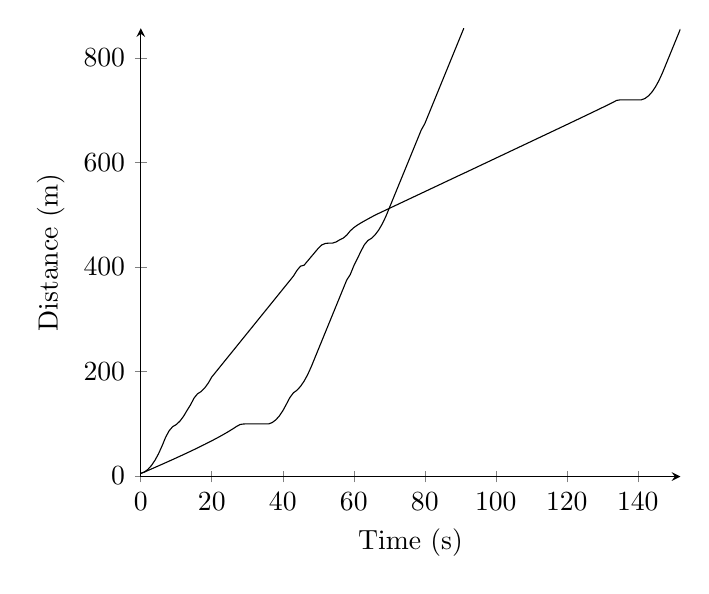
\begin{tikzpicture}
\begin{axis}[
legend style={anchor=west},
axis x line=bottom,
axis y line=left,
ymin=-1,
xlabel=Time (s),
ylabel=Distance (m),
]
\addplot[] coordinates {
(0, 5.1)
(1, 7.6)
(2, 10.551264739)
(3, 13.5148458518)
(4, 16.491720024)
(5, 19.4829705626)
(6, 22.4898024406)
(7, 25.5135599774)
(8, 28.555747716)
(9, 31.6180551961)
(10, 34.7023865031)
(11, 37.810895714)
(12, 40.9460296665)
(13, 44.1105798987)
(14, 47.3077461535)
(15, 50.5412145976)
(16, 53.8152549271)
(17, 57.1348419561)
(18, 60.5058092771)
(19, 63.9350454196)
(20, 67.4307470306)
(21, 71.0027496137)
(22, 74.6629653545)
(23, 78.4259712621)
(24, 82.309812202)
(25, 86.3371174595)
(26, 90.5366852977)
(27, 94.9457842613)
(28, 98.6044896023)
(29, 99.6320158223)
(30, 99.7193641886)
(31, 99.7193641886)
(32, 99.7193641886)
(33, 99.7193641886)
(34, 99.7193641886)
(35, 99.7193641886)
(36, 99.7193641886)
(37, 102.219364189)
(38, 107.219364189)
(39, 114.719364189)
(40, 124.719364189)
(41, 137.219364189)
(42, 150.125095958)
(43, 159.234657451)
(44, 164.142641251)
(45, 171.550625052)
(46, 181.458608852)
(47, 193.866592652)
(48, 208.774576453)
(49, 225.374576453)
(50, 241.974576453)
(51, 258.574576453)
(52, 275.174576453)
(53, 291.774576453)
(54, 308.374576453)
(55, 324.974576453)
(56, 341.574576453)
(57, 358.174576453)
(58, 374.774576453)
(59, 385.384576453)
(60, 401.984576453)
(61, 415.584576453)
(62, 429.92347141)
(63, 442.651450477)
(64, 450.734866052)
(65, 454.801722929)
(66, 461.368579805)
(67, 470.435436682)
(68, 482.002293558)
(69, 496.069150435)
(70, 512.636007311)
(71, 529.236007311)
(72, 545.836007311)
(73, 562.436007311)
(74, 578.936007311)
(75, 595.536007311)
(76, 612.136007311)
(77, 628.736007311)
(78, 645.336007311)
(79, 661.936007311)
(80, 674.076007311)
(81, 690.676007311)
(82, 707.276007311)
(83, 723.876007311)
(84, 740.476007311)
(85, 757.076007311)
(86, 773.676007311)
(87, 790.276007311)
(88, 806.876007311)
(89, 823.476007311)
(90, 840.076007311)
(91, 856.676007311)
};
\addplot[] coordinates {
(0, 5.1)
(1, 7.6)
(2, 12.6)
(3, 20.1)
(4, 30.1)
(5, 42.6)
(6, 57.6)
(7, 74.2)
(8, 86.6997297278)
(9, 94.5649106955)
(10, 98.4573862023)
(11, 104.849861709)
(12, 113.742337216)
(13, 125.134812723)
(14, 136.02728823)
(15, 149.039719459)
(16, 157.36882852)
(17, 161.634015209)
(18, 168.399201898)
(19, 177.664388587)
(20, 189.429575276)
(21, 197.822653454)
(22, 206.215777321)
(23, 214.6089514)
(24, 223.002180831)
(25, 231.39547148)
(26, 239.788830074)
(27, 248.182264361)
(28, 256.575783316)
(29, 264.969397389)
(30, 273.363118827)
(31, 281.756962071)
(32, 290.150944275)
(33, 298.545085976)
(34, 306.939411965)
(35, 315.333952455)
(36, 323.728744648)
(37, 332.123834879)
(38, 340.519281603)
(39, 348.915159643)
(40, 357.311566345)
(41, 365.708630755)
(42, 374.106527678)
(43, 382.505499944)
(44, 393.404472211)
(45, 401.495043603)
(46, 403.315921389)
(47, 411.406228382)
(48, 419.498021114)
(49, 427.592671136)
(50, 435.692811781)
(51, 442.135492037)
(52, 444.939362145)
(53, 445.562177829)
(54, 445.594416168)
(55, 447.718518537)
(56, 451.744076421)
(57, 455.010741568)
(58, 460.777406715)
(59, 468.983220762)
(60, 475.126173639)
(61, 479.98217806)
(62, 484.165440335)
(63, 488.045666837)
(64, 491.801513568)
(65, 495.508625682)
(66, 499.197053628)
(67, 502.398679294)
(68, 505.60038685)
(69, 508.802179833)
(70, 512.00406199)
(71, 515.206037288)
(72, 518.408109936)
(73, 521.610284397)
(74, 524.812565414)
(75, 528.014958028)
(76, 531.217467605)
(77, 534.420099859)
(78, 537.622860883)
(79, 540.825757181)
(80, 544.028795704)
(81, 547.231983886)
(82, 550.43532969)
(83, 553.638841654)
(84, 556.842528945)
(85, 560.046401418)
(86, 563.250469681)
(87, 566.454745168)
(88, 569.659240225)
(89, 572.863968196)
(90, 576.068943533)
(91, 579.17418191)
(92, 582.384466492)
(93, 585.594782946)
(94, 588.80513343)
(95, 592.015520299)
(96, 595.225946133)
(97, 598.436413761)
(98, 601.646926294)
(99, 604.857487159)
(100, 608.068100143)
(101, 611.278769439)
(102, 614.489499704)
(103, 617.700296122)
(104, 620.911164487)
(105, 624.122111289)
(106, 627.333143825)
(107, 630.54427033)
(108, 633.755500132)
(109, 636.966843838)
(110, 640.178313567)
(111, 643.389923225)
(112, 646.601688852)
(113, 649.81362905)
(114, 653.025765514)
(115, 656.238123711)
(116, 659.450733742)
(117, 662.663631452)
(118, 665.876859877)
(119, 669.090471166)
(120, 672.304426716)
(121, 675.540738148)
(122, 678.778922376)
(123, 682.019357719)
(124, 685.262533559)
(125, 688.509095201)
(126, 691.759912938)
(127, 695.016192554)
(128, 698.279660573)
(129, 701.552893549)
(130, 704.839949662)
(131, 708.147712295)
(132, 711.489214454)
(133, 714.894166483)
(134, 718.464164333)
(135, 719.59368241)
(136, 719.699074378)
(137, 719.699074378)
(138, 719.699074378)
(139, 719.699074378)
(140, 719.699074378)
(141, 719.699074378)
(142, 722.199074378)
(143, 727.199074378)
(144, 734.699074378)
(145, 744.699074378)
(146, 757.199074378)
(147, 772.199074378)
(148, 788.799074378)
(149, 805.399074378)
(150, 821.999074378)
(151, 838.599074378)
(152, 855.199074378)
};

\end{axis}
\end{tikzpicture}
\label{tik:distance:100:53}
\caption{100 percent diving with GSC on route $53$}
\end{figure}

%\begin{tikzpicture}\begin{axis}
};
\addplot+[ycomb] coordinates{
(216, 52.252945617)
(217, 10.2835247016)
(214, 16.2856718575)
(215, 4.51864792679)
(213, 28.3873548357)
(211, 11.189338998)
(264, 40.4878802965)
(218, 0)
(219, 22.2220848566)
(133, 0)
(132, 34.4508958132)
(131, 28.3594198907)
(130, 22.1385166496)
(137, 0)
(135, 4.50616611369)
(165, 16.2267027888)
(139, 28.285187868)
(225, 52.3061097447)
(25, 16.0530002679)
(26, 10.1475132786)
(167, 52.905635371)
(20, 4.06070836139)
(21, 0)
(95, 16.7780005237)
(28, 13.0397800766)
(29, 0)
(178, 40.1749084596)
(0, 0.887926285604)
(221, 11.0667215168)
(281, 28.1590830651)
(8, 0.879701275233)
(96, 10.9849476286)
(284, 33.0003184931)
(68, 7.55165507934)
(87, 7.01750211778)
(119, 22.4988880985)
(263, 0)
(121, 40.2128463437)
(261, 22.2161474214)
(124, 22.5816882433)
(265, 0)
(127, 34.5048855528)
(128, 0)
(129, 52.6828088003)
(269, 16.4398851063)
(268, 22.2261723856)
(183, 16.8024845352)
(59, 4.06105996166)
(58, 4.32362219439)
(55, 4.10269772145)
(54, 8.12141482104)
(227, 28.5551151413)
(50, 8.38010669551)
(53, 0)
(259, 22.7745844792)
(298, 0)
(296, 4.31694972892)
(297, 40.4553565181)
(294, 40.1480987865)
(295, 22.2334499586)
(292, 40.1264458833)
(293, 16.9100041831)
(291, 40.5409654352)
(199, 4.35555745706)
(66, 20.4512404622)
(134, 28.6189430663)
(194, 0)
(197, 10.2047254435)
(196, 21.1414626766)
(191, 16.8319208832)
(190, 22.5846717422)
(271, 0)
(273, 34.2295001485)
(111, 11.3590799416)
(275, 10.3466370086)
(276, 28.1627318956)
(82, 22.718673814)
(279, 16.198959792)
(81, 28.2427318469)
(86, 22.1371668922)
(175, 10.9783281237)
(84, 52.7044109674)
(85, 5.04021199249)
(251, 34.3955366687)
(140, 28.580112231)
(108, 4.326167767)
(173, 34.2552838173)
(141, 16.7396435688)
(172, 40.6837062669)
(27, 0)
(3, 1.04420549155)
(255, 22.6172191574)
(24, 10.0531682208)
(245, 10.8464242737)
(244, 0)
(247, 0)
(241, 16.8271854495)
(240, 24.9439593649)
(243, 11.0294469892)
(102, 10.3777836793)
(103, 4.39269776309)
(100, 58.715030228)
(101, 30.8873579857)
(249, 16.738667879)
(104, 40.4248832298)
(105, 22.6658469812)
(39, 16.0389462527)
(38, 9.97543373366)
(33, 0)
(32, 8.33961614558)
(224, 22.6943008186)
(30, 20.3718391591)
(37, 22.1587029266)
(35, 2.38991943591)
(252, 5.22601443101)
(64, 22.13130224)
(65, 0)
(179, 0)
(67, 0)
(177, 0)
(69, 2.47903564849)
(174, 10.3127546711)
(256, 34.4823477755)
(257, 22.7308631355)
(170, 34.098783136)
(203, 52.7582624606)
(253, 52.6262542806)
(182, 10.8682501666)
(195, 34.4655481847)
(180, 10.3224731989)
(2, 0.889785751671)
(186, 5.31367419411)
(187, 22.7052298423)
(185, 16.1605886549)
(188, 45.0508173792)
(189, 40.3306851983)
(202, 34.2922024545)
(4, 0.858119596325)
(120, 34.5436475256)
(6, 6.26091222826)
(57, 0)
(99, 52.2575951587)
(168, 22.4135028295)
(169, 5.13775554004)
(229, 10.295455161)
(228, 34.5018262923)
(164, 0)
(92, 28.1764589812)
(160, 16.7564116485)
(162, 16.1825565598)
(11, 11.8283948176)
(10, 0.881112011558)
(13, 1.06146657052)
(12, 6.31020600882)
(15, 0.875296659051)
(14, 58.6672268685)
(17, 0.993840898557)
(16, 6.22794134696)
(19, 0.888781204593)
(18, 6.20293203127)
(118, 34.3543907429)
(88, 10.34819743)
(116, 34.7586327154)
(274, 58.6919651903)
(151, 27.1786828977)
(153, 28.7878919466)
(152, 28.1038034905)
(155, 28.2228618291)
(154, 34.4696486913)
(157, 28.5873349819)
(156, 16.775155837)
(159, 22.6084045705)
(158, 10.8361840758)
(62, 15.9833105543)
(277, 28.2764304681)
(90, 13.1217001857)
(238, 58.7327045428)
(235, 28.6501799394)
(237, 28.5527321263)
(231, 10.8267935469)
(232, 34.3695501862)
(233, 22.445048936)
(280, 10.2601636215)
(48, 3.93928596866)
(46, 0)
(44, 14.3903646534)
(45, 10.0088845232)
(42, 0)
(40, 14.5185355396)
(1, 6.44158771882)
(5, 6.33155562465)
(9, 6.23692159842)
(200, 34.5846228307)
(144, 10.3377609298)
(145, 16.728360112)
(142, 4.4518685762)
(204, 58.7375726484)
(207, 10.8693114242)
(209, 22.3262391201)
(149, 23.0494155894)
(77, 16.2953052439)
(74, 16.2546317465)
(106, 40.1412078513)
(72, 40.6167688582)
(71, 19.1793620961)
(70, 5.12135647663)
(79, 5.24282483604)
(78, 28.596095633)
(122, 16.2074955811)
(270, 52.4359425241)
(89, 0)
(267, 34.2918595684)
(126, 28.5503390242)
\addplot+[ycomb] coordinates{
(210, 28.1097793763)
(210, 0)
(136, 52.2280479547)
(136, 0)
(138, 34.3467427786)
(138, 0)
(198, 34.6152811937)
(198, 0)
(22, 20.3266947089)
(22, 10.0447349346)
(289, 40.1976509476)
(289, 22.7168289734)
(283, 58.6320978831)
(283, 4.31438946042)
(123, 52.7292763657)
(123, 0)
(125, 19.7400405749)
(125, 0)
(56, 13.7112306443)
(56, 0)
(52, 19.8176908191)
(52, 4.04307309312)
(146, 58.5827933491)
(146, 34.6907037185)
(147, 34.1110400653)
(147, 16.2145455372)
(193, 52.8336680281)
(193, 0)
(80, 34.1002985828)
(80, 3.24308949069)
(254, 10.5251603275)
(254, 0)
(242, 58.5806667528)
(242, 4.87870006484)
(161, 34.2151874165)
(161, 0)
(34, 22.0585066331)
(34, 2.49293574307)
(246, 53.011035511)
(246, 0)
(94, 28.2491635302)
(94, 10.727029223)
(61, 13.312000988)
(61, 0)
(258, 22.6217152778)
(258, 5.01039621943)
(171, 52.3163917096)
(171, 9.55366723979)
(272, 10.8338464926)
(272, 0)
(181, 34.151374051)
(181, 16.5489447218)
(248, 52.6363940379)
(248, 0)
(97, 52.6547729656)
(97, 28.6648254432)
(98, 40.2593862116)
(98, 3.21946066682)
(222, 52.6819066117)
(222, 5.23552143383)
(93, 16.3158568778)
(93, 0)
(287, 16.7670833498)
(287, 0)
(31, 34.255056387)
(31, 2.44722481145)
(150, 58.7435786763)
(150, 4.41595408894)
(113, 28.6293422449)
(113, 10.9734549893)
(278, 52.6666260662)
(278, 0)
(83, 52.4478526303)
(83, 40.1971805753)
(234, 22.8473160709)
(234, 10.8390960135)
(236, 50.4031601251)
(236, 10.3285979681)
(230, 58.8696240113)
(230, 15.341659667)
(49, 26.3558240891)
(49, 0)
(47, 16.0158863142)
(47, 0)
(43, 27.9870688156)
(43, 0)
(208, 28.1330483343)
(208, 10.7370070602)
(148, 16.2311692676)
(148, 4.29963387855)
(76, 52.2595937482)
(76, 0)
(75, 52.6464795668)
(75, 5.15014459374)
(112, 34.4737051594)
(112, 16.80717737)
(262, 52.3174756198)
(262, 28.7833548519)
(260, 40.2876209009)
(260, 0)
(266, 52.2325690044)
(266, 0)
\addplot+[ycomb] coordinates{
(285, 28.5350456998)
(285, 16.5886687888)
(285, 0)
(115, 34.5913828471)
(115, 22.27329098)
(115, 4.69795317646)
(176, 52.7187685594)
(176, 31.7604481719)
(176, 16.3285637619)
};
\end{axis}\end{tikzpicture}

\subsection{Fuel Consumption}
The purpose of \tech is to reduce the fuel consumption at least for the vehicles using the system. 
We use SUMO's build-in function to calculate the vehicles fuel consumption, which is explained in \cite{SUMOFuel}.

The total fuel consumption for all vehicles in the network is plotted in Figure~\ref{fig:TestResults:fuelTotal}.
Figure~\ref{fig:TestResults:fuelTotal} plots the fuel consumption for all vehicles in the network for two different simulations: one where all vehicles use \tech (blue) and one where no vehicles are using \tech (green).
The average fuel consumption when all vehicles use \tech is about $77 ml$, and about $108 ml$ when no one use \tech.
We therefore see a significant overall reduction in fuel consumption in this setting if \tech is used by everybody.
Looking at just the selected route through the network, we see the same tendency (see Figure~\ref{fig:TestResults:fuelRoute}). 
The average fuel consumption with \tech is about $114 ml$ and about $166 ml$ without. 
\begin{figure}[h]
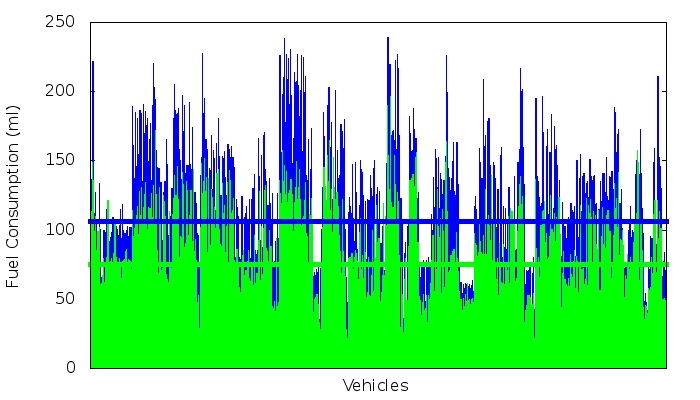
\includegraphics[width=0.5\textwidth]{images/tp0/fuelTotal.png}
\caption{Fuel consumption for all vehicles in the network. Blue: 100\% use \tech, green: 0\% use \tech}
\label{fig:TestResults:fuelTotal}
\end{figure}
\begin{figure}[h]
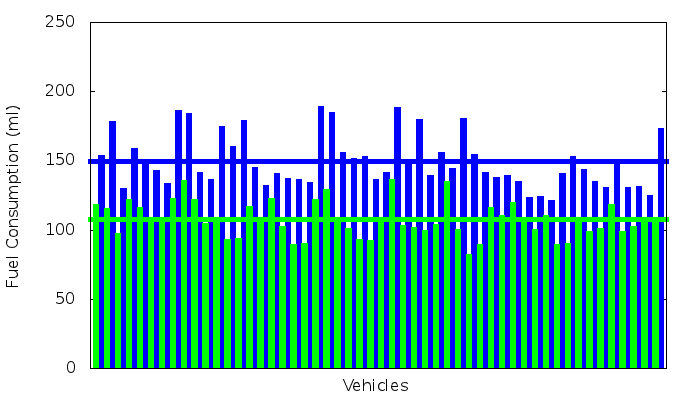
\includegraphics[width=0.5\textwidth]{images/tp0/fuelRoute.png}
\caption{Fuel consumption for all vehicles on the selected route}
\label{fig:TestResults:fuelRoute}
\end{figure}

It is, however, also interesting to investigate the influence \tech has when only a few drivers use it.
Figure~\ref{fig:TestResults:fuelControlled10} and~\ref{fig:TestResults:fuelUncontrolled10} plot the fuel consumption for 10\% of the vehicles are using \tech.
Figure~\ref{fig:TestResults:fuelControlled10} shows the 10 \% using \tech, and Figure~\ref{fig:TestResults:fuelUncontrolled10} show the 90 \% not using \tech.
We see that the average fuel consumption is about $119 ml$ for the 10 \% using \tech, and about $168$ for the 90 \% not using it.
The fuel consumption is less for those who use \tech, and the fuel consumption is only increased by $1 ml$ for those who do not use \tech compared to the situation where no vehicles used \tech.
We see the same results when 50 \% of the vehicles use \tech.

We can therefore conclude that in the tested use case, we see a significate reduction in fuel consumption even when it is only implemented in a small subset of the vehicles. 
Moreover, vehicles using \tech does not have a negative influence the other fuel consumption of the vehicles.

\begin{figure}[h]
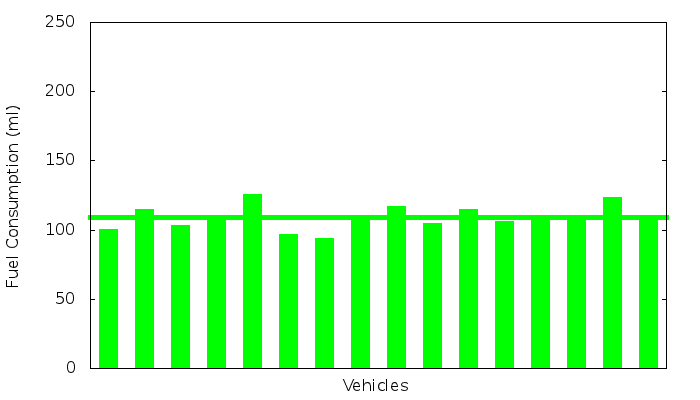
\includegraphics[width=0.5\textwidth]{images/tp0/fuelRouteControlled10.png}
\caption{Fuel consumption for the 10 \% of the vehicles driving with \tech on the selected route}
\label{fig:TestResults:fuelControlled10}
\end{figure}
\begin{figure}[h]
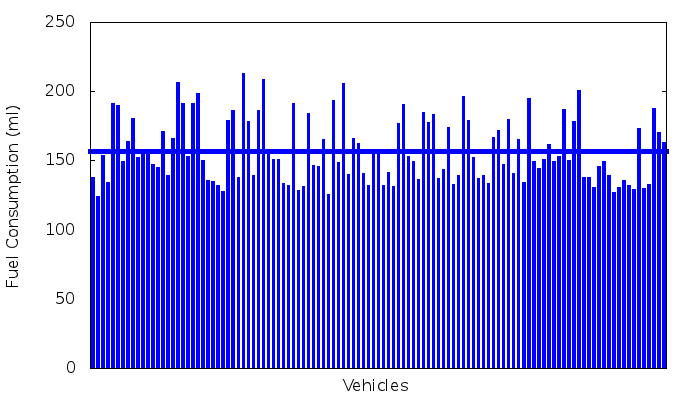
\includegraphics[width=0.5\textwidth]{images/tp0/fuelRouteUncontrolled10.png}
\caption{Fuel consumption for the 90 \% of the vehicles driving without \tech on the selected route}
\label{fig:TestResults:fuelUncontrolled10}
\end{figure}

\subsection{Distance}
Figure~\ref{fig:TestResults:distance100} shows the distance vehicles drive on the selected route as a function of time when their driving behaviour is solely controlled by SUMO. 
The vehicle is stationary whenever the curve flatens.
From the figure we clearly see that the vehicles on this route has to stop four times, at 250 meter, at 550 meters, at 750 meters and again at 1100 metets.

When we control the speed of the vehicles using \tech, we see a different result showed in Figure~\ref{fig:TestResults:distance100}.
The curves in this figure are much more smooth, and fewer vehicles has to stop completely at a cross section.
Some vehicles have to stop due to blocking vehicles or cross traffic, which we do not take into account.

We can therefore see that using \tech results in less full stops.

The results of introducing the system to 10\% of the vehicles can be seen in Figure~\ref{fig:TestResults:distanceUnC10}. 
The remaning 90\% is for the most part unaffected by the system. 
There is a few instances where uncontrolled vehicles are forced to slow down and stay behind a slower moving vehicle using the system.

\begin{figure}[H]
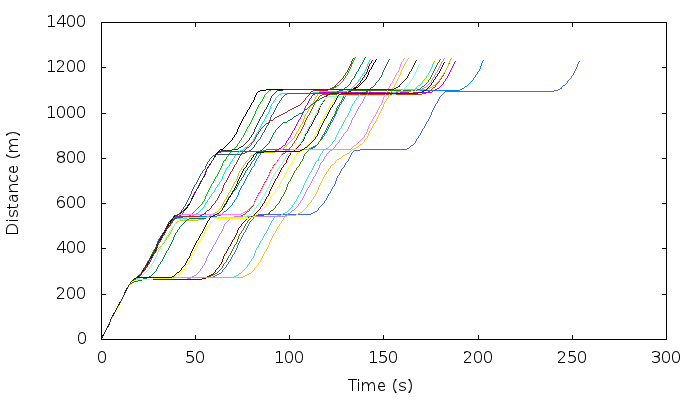
\includegraphics[width=0.5\textwidth]{images/tp0/distanceUncontrolled10.png}
\caption{Travel distance for the 90 \% of the vehicles driving without \tech on the selected route}
\label{fig:TestResults:distanceUnC10}
\end{figure}

\begin{figure}[H]
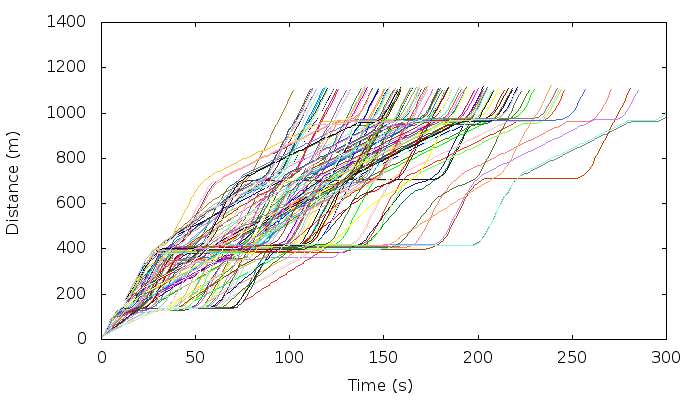
\includegraphics[width=0.5\textwidth]{images/tp0/distanceControlled100.png}
\caption{Travel distance of vehicles when all drive with \tech on the selected route}
\label{fig:TestResults:distance100}
\end{figure}

\subsection{Speed}
Figure~\ref{fig:TestResults:speed0} shows the speed at which SUMO controlled vehicles on the selected route drive as a function over time.
The graph clearly shows that the vehicles quicly accelerates up to the maximal speed, then quickly decelerates to a full stop and then quickly accelerates again.
By using \tech we see a very different outline (See Figure~\ref{fig:TestResults:speed100}).
Few vehicles decelerates to $0\ km/h$, and most stay above $14\ km/h$.

Again, the result of introducing the system to 10\% of the vehicles can be seen in Figure \ref{fig:TestResults:speedUnC10}. 
The remaning 90\% is almoste unaffected by the system.

\begin{figure}[H]
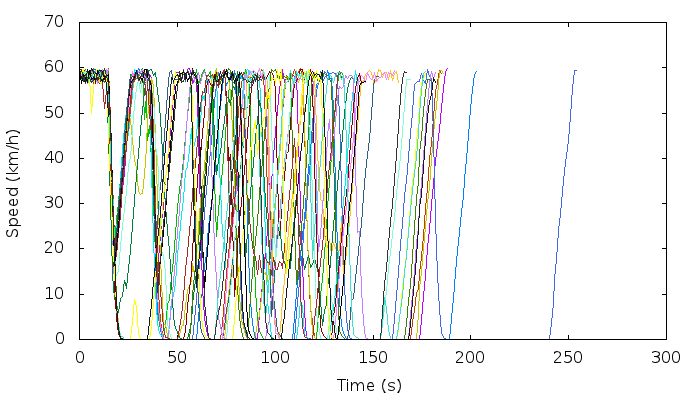
\includegraphics[width=0.5\textwidth]{images/tp0/speedUncontrolled10.png}
\caption{Speed for the 90 \% of the vehicles driving without \tech on the selected route}
\label{fig:TestResults:speedUnC10}
\end{figure}

\begin{figure}[H]
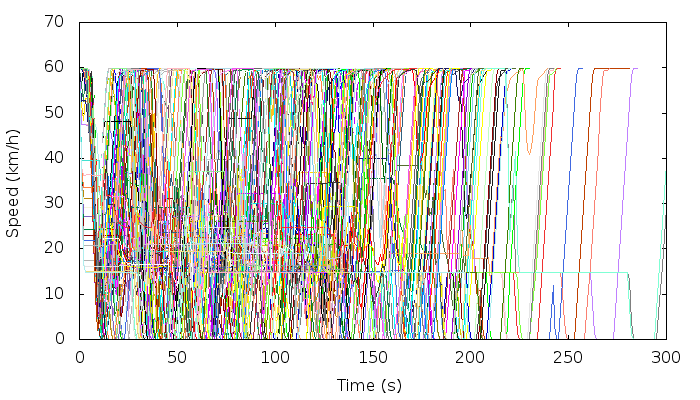
\includegraphics[width=0.5\textwidth]{images/tp0/speedControlled100.png}
\caption{Speed of vehicles when all drive with \tech on the selected route}
\label{fig:TestResults:speed100}
\end{figure}


\subsection{Time}
%TODO: Find error in these results. They are all 100.
\begin{comment}
It is interesting to investigate whether driving with \tech results in a longer travel time than without.


It takes on average 100 seconds to drive through the network on any route in our test without \tech, and when all vehicles drive with \tech it takes 77 seconds. 

We therefore do not see any significant differens in thees results.
\end{comment}

